% !TeX encoding = UTF-8
% !TeX program = pdflatex
% !BIB program = bibtex


\documentclass[english]{lni}
\usepackage[backend=biber]{biblatex}
\usepackage{float}
\usepackage{mathtools}
%\newcommand{\argmax}{\operatornamewithlimits{arg\,max}}
%\newcommand{\argmin}{\operatornamewithlimits{arg\,min}}

\defbibfilter{bookorarticleormisc}{%
    \type{book} \or \type{article} \or \type{misc}
}
\bibliography{references} %\printbibliography if you use biblatex/Biber

\begin{document}

\title[Word and Document Embeddings]{Word and Document Embeddings}
\author[Atanas Denkov]
{Atanas Denkov\footnote{Hochschule für Technik und Wirtschaft, Angewandte Informatik, Wilhelminenhofstr., 12459 Berlin,
Germany \email{s0559025@htw-berlin.de}}}

\maketitle

\begin{abstract}
TODO
\end{abstract}
    
\begin{keywords}
    Machine Learning \and Distributed Computing \and Self-organizing Maps \and Unsupervised Learning %Keyword1 \and Keyword2
\end{keywords}

%%% Beginn des Artikeltexts
%%\section{Introduction}
%%\section{Related Work}
\clearpage
\section{Continuous Bag of Words}
\begin{figure}[H]
    \centering
    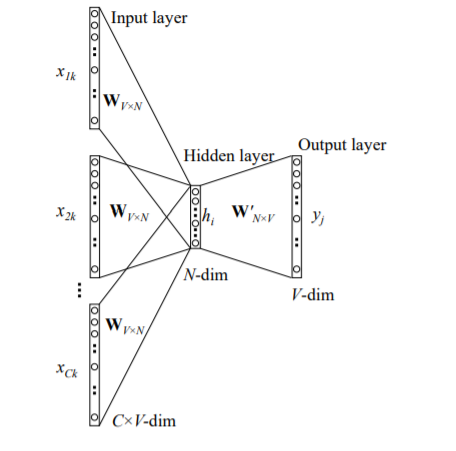
\includegraphics[width=0.70\textwidth]{images/word2vec-arch.PNG}
    \caption{The Continuous Bag of Words model}
    \label{fig:word2vec-arch}
\end{figure}
The Continuous Bag of Words model is a shallow neural network used for creating word vectors, also refered to as word \textit{embeddings}. 
The set of word vectors forms a vector space that captures the similarity between words. 
The objective of the model is to predict the true center word $w_o$ given the context words $w_{1}, w_{2},\hdots, w_{c}$ that surround it. 
For example, in the sentence \textit{The big brown fox jumped over the puddle}, we would like to predict the word \textit{jumped} given 
the context words \textit{[the, big, brown, over, the, puddle]}.
The algorithm takes a probabilistic approach and tries to model the probability $p(w_{o}|w_{1}, w_{2},\hdots, w_{c})$. 
The objective is then formulated as maximizing that probability.\\
\subsection{Forward pass}
The input to our model is a set of context words represented as one-hot encoded vectors $x_{1}, x_{2},\hdots,x_{c}$ where $x_{c} \in \mathbb{R}^{V}$.
$V$ corresponds to the size of the vocabulary that the model can perceive. 
Each one-hot vector has a $1$ at the index that is unique to the word it represents ($x_{k} = 1$) and $0$'s everywhere else ($\{x_{k'} = 0 | k'\in [1,2,\hdots,V], k' \neq k\}$).
The neural network has a hidden matrix $\textbf{W} \in \mathbb{R}^{V \times N}$ that holds a word vector $v_w \in \mathbb{R}^N$ for each word $w$ when it appears as a context word.
Given that the context words are the input to our model, this matrix is called the \textit{input matrix}. 
The hidden layer of the network functions as a lookup table to extract the input vectors $v_1, v_2,\hdots,v_c$ by computing the following dot products
\begin{align}
    v_1 &= \textbf{W}^{T}x_1 \nonumber \\
    v_2 &= \textbf{W}^{T}x_2 \nonumber \\
        & \vdots                       \\
    v_c &= \textbf{W}^{T}x_c. \nonumber
\end{align}
These vectors are then averaged to form the hidden state 
\begin{equation}
    \label{eq:hidden_state}
    \textbf{h} = \frac{1}{C}(v_1 + v_2 + \hdots + v_c), \:
    \textbf{h} \in \mathbb{R}^{N}.
\end{equation}
$N$ denotes the size of the embedding space and is typically a hyperparameter. 
The model has an additional weight matrix $\textbf{W'} \in \mathbb{R}^{N \times V}$ that holds a word vector $v'_w \in \mathbb{R}^N$ for each word $w$ when it appears 
as a center word. We refer to this matrix as the \textit{output matrix}.
If we compute the dot product between the hidden state $\textbf{h}$ and a word vector $v'_j$,
we obtain a score that measures the similarity between the context and the word represended by that word vector.
\begin{equation}
    u_{j} = {v'_{j}}^{T}\textbf{h}
\end{equation}
We convert the scores into probabilities via the softmax function and obtain our prediction
\begin{align}
    \label{eq:yhat}
    p(w_{j}|w_{I}) = \hat{y}_{j} = \frac{\exp{u_{j}}}{\sum_{j'=1}^{V}{\exp{u_{j'}}}} = \frac{\exp{{v'_{j}}^{T}\textbf{h}}}{\sum_{j'=1}^{V}{\exp{{v'_{j'}}^{T}\textbf{h}}}}. 
\end{align}
\subsection{Backward pass}
The objective of our model is to maximize the probability $p(w_{j}|w_{I})$ defined in Equation \ref{eq:yhat} when 
$w_{j}$ really is the center word given the context $w_{I}$. That is, we want to compare the target probability $y_{j} = 1$ 
with our estimate $\hat{y}_{j}$. We do this by using a simplified version of the cross-entropy loss function 
\begin{align}
    H(\hat{y}_{j}, y_{j}) &= -y_{j}\log{\hat{y}_{j}} \nonumber \\ 
    &= -\log{\hat{y}_{j}}  \nonumber \\ 
    &= -\log{\frac{\exp{u_{j}}}{\sum_{j'=1}^{V}{\exp{u_{j'}}}}} \label{eq:logtrans1} \\
    &= -u_{j} + \log{\sum_{j'=1}^{V}{\exp{u_{j'}}}} \label{eq:logtrans2}.
\end{align}
The transition from (\ref{eq:logtrans1}) to (\ref{eq:logtrans2}) follows the logarithm rule for fractions
\begin{equation}
    \log_{b}{(\frac{A}{B})} = \log_{b}{(A)} - \log_{b}{(B)}.
\end{equation}
We use gradient descent to update $v'_j$ and $v_{1}, v_{2}\hdots,v_{c}$ such that $H(\hat{y}_{j}, y_{j}) \approx 0$.\\
The chain rule tells us that 
\begin{equation}
    \label{eq:der1}
    \frac{\partial H}{\partial v'_{j}} = \frac{\partial H}{\partial u_{j}}\cdot\frac{\partial u_{j}}{\partial v'_{j}}.
\end{equation}
Calculating the derivative of the loss yields
\begin{align}
    \frac{\partial H}{\partial u_{j}} &= \frac{\partial}{\partial u_{j}}-u_{j} + \log{\sum_{j'=1}^{V}{\exp{u_{j'}}}} \nonumber \\
    &= \frac{\partial}{\partial u_{j}}-u_{j} + \frac{\partial}{\partial u_{j}}\log{\sum_{j'=1}^{V}{\exp{u_{j'}}}} \nonumber \\
    &= -1 + \frac{1}{\sum_{j'=1}^{V}{\exp{u_{j'}}}}\frac{\partial}{\partial u_{j}}\sum_{j'=1}^{V}{\exp{u_{j'}}} \nonumber \\
    &= -1 + \frac{1}{\sum_{j'=1}^{V}{\exp{u_{j'}}}}\frac{\partial}{\partial u_{j}}\exp{u_{j}} \nonumber \\ 
    &= -1 + \frac{\exp{u_{j}}}{\sum_{j'=1}^{V}{\exp{u_{j'}}}} \nonumber \\ 
    &= \hat{y}_{j} - 1.
\end{align}
Next we take the derivative of $u_{j}$ with respect to $v'_{j}$.
\begin{equation}
    \label{eq:hiddenvder}
    \frac{\partial u_{j}}{\partial v'_{j}} = \frac{\partial}{\partial v'_{j}}v'_{j}\cdot\textbf{h} = \textbf{h}.
\end{equation}
By substituting our calculations in Equation \ref{eq:der1} and considering that the index of the true center word is $j$, then 
our derivative is 
\begin{equation}
\frac{\partial H}{\partial v'_{j'}} = 
\begin{dcases}
    (\hat{y}_{j'}-1)\cdot\textbf{h},& \text{if } j'=j\\
    (\hat{y}_{j'})\cdot\textbf{h} & \text{otherwise.}
\end{dcases}
\end{equation}
Since we are using gradient descent, our update rule for $v'_{j'}$ becomes 
\begin{equation}
\label{eq:vjder1}
{v'_{j'}}^{(new)} = 
\begin{dcases}
    {v'_{j'}}^{(old)} - \alpha\cdot((\hat{y}_{j'}-1)\cdot\textbf{h}),& \text{if } j'=j\\
    {v'_{j'}}^{(old)} - \alpha\cdot\hat{y}_{j'}\cdot\textbf{h} & \text{otherwise.}
\end{dcases}
\end{equation}
Note that when $j' = j$, the negative sign of the expression $\hat{y}_{j'}-1$ cancels out the negative sign of the update rule, thus 
pushing the value of $v'_{j}$ towards the context $\textbf{h}$. Conversely, when $j' \neq j$, the output vector is pushed away from the context. 
In other words, vectors that have similar contexts are clustered together by being pushed away from unrelated contexts and at the same time being pushed towards contexts that are
meaningful. This notion is refered to as \textit{distributional semantics}.\\
The next step is to compute the partial derivatives of the loss function with respect to the input vectors $v_1, v_2,\hdots,v_c$.
The chain rule tells us that 
\begin{equation}
    \label{eq:der2}
    \frac{\partial H}{\partial v_i} = \sum_{j = 1}^{V}{\frac{\partial H}{\partial u_{j}}\cdot\frac{\partial u_{j}}{\partial \textbf{h}}\cdot\frac{\partial \textbf{h}}{\partial v_{i}}}, \: \text{for} \: i \in [1, 2, \hdots, C].
\end{equation}
The first derivative in the summation has already been computed. The second one yields
\begin{equation}
    \label{eq:subder1}
    \frac{\partial u_{j}}{\partial \textbf{h}} = \frac{\partial}{\partial \textbf{h}}{v'_{j}}^{T}\textbf{h} = v'_{j},
\end{equation}
and the third one:
\begin{equation}
    \label{eq:subder2}
    \frac{\partial \textbf{h}}{\partial v_{i}} = \frac{\partial}{\partial v_{i}} \frac{1}{C}(v_1 + v_2 + \hdots + v_c) = \frac{1}{C}.
\end{equation}
Substituting (\ref{eq:subder1}) and (\ref{eq:subder2}) into (\ref{eq:der2}) gives us
\begin{equation}
\frac{\partial H}{\partial v_i} =
\begin{dcases}
    \frac{1}{C}\cdot \sum_{j' = 1}^{V}{(\hat{y}_{j'}-1)\cdot v'_{j'}},& \text{if } j'=j\\
    \frac{1}{C}\cdot \sum_{j' = 1}^{V}{\hat{y}_{j'}\cdot v'_{j'}} & \text{otherwise.}
\end{dcases}
\; \text{for} \: i \in [1, 2, \hdots, C]
\end{equation}
We now derive the update rule 
\begin{equation}
\label{eq:ctxder}
{v_{i}}^{(new)} = 
\begin{dcases}
    {v_{i}}^{(old)} - \alpha\cdot \frac{1}{C}\cdot \sum_{j' = 1}^{V}{(\hat{y}_{j'}-1)\cdot v'_{j'}},& \text{if } j'=j\\
    {v_{i}}^{(old)} - \alpha\cdot \frac{1}{C}\cdot \sum_{j' = 1}^{V}{\hat{y}_{j'}\cdot v'_{j'}} & \text{otherwise.}
\end{dcases}
\; \text{for} \: i \in [1, 2, \hdots, C]
\end{equation}
\subsection{Optimization}
Notice that Equation \ref{eq:yhat} requires iterating over the whole vocabulary to compute the normalization factor.
The vocabulary usually exceeds hundreds of thousands of words, which renders this computation rather inefficient.
A technique called \textit{negative sampling} deals with this by reformulating the objective function, the weights and the update equations.
Instead of going over the whole vocabulary, we can sample a set of words from it that are unlikely to occur near the context and update their 
weights in such a way that they are pushed further away from the context, while the true center word is pushed towards it.\\
First, we remodel the objective function to be 
\begin{equation}
    H(\hat{y}_{j}, y_{j}) = -\log{\sigma(u_{j})} - \sum_{k = 1}^{K}{\log{\sigma(-u_{k})}}.
\end{equation}
The words $\{u_{k}|k \in [1, 2,\hdots,K]\}$ are sampled from a noise distribution $P(w)$, which is defined in terms of word frequencies.
A good heuristic value for $K$ is 10. Note that $K$ is a lot smaller than $V$.
If $f(w)$ defines the relative frequency of the word $w$ in our corpus, then the probability of using $w$ as a negative sample is defined by
\begin{equation}
    P(w) = \frac{{f(w)}^{3/4}}{\sum_{i = 1}^{V}{{f(w_{i})}^{3/4}}}.
\end{equation}
The power factor $3/4$ is determined heuristically and tends to favor words that appear less frequently.\\
Now that we have changed the objective, we need to recalculate the partial derivatives for our weights.
Backpropagating the update signal to the output vector $v'_{j}$ is done via the following derivative chain:
\begin{equation}
    \frac{\partial H}{\partial v'_{j}} = \frac{\partial H}{\partial \sigma(u_{j})} \cdot \frac{\partial \sigma(u_{j})}{\partial u_{j}} \cdot \frac{\partial u_{j}}{\partial v'_{j}}.
\end{equation}
The first derivative yields
\begin{align}
    \frac{\partial H}{\partial \sigma(u_{j})} &= \frac{\partial}{\partial \sigma(u_{j})}-\log{\sigma(u_{j})} - \sum_{k = 1}^{K}{\log{\sigma(-u_{k})}} \nonumber \\ 
    &= \frac{\partial}{\partial \sigma(u_{j})}-\log{\sigma(u_{j})} - \frac{\partial}{\partial \sigma(u_{j})} \sum_{k = 1}^{K}{\log{\sigma(-u_{k})}} \nonumber \\
    &= -\frac{1}{\sigma(u_{j})} \frac{\partial}{\partial \sigma(u_{j})} \sigma(u_{j}) \nonumber \\ 
    &= -\frac{1}{\sigma(u_{j})}.
\end{align}
The derivative of the sigmoid function is defined as 
\begin{equation}
    \frac{\partial \sigma(u_{j})}{\partial u_{j}} = \sigma(u_{j})\cdot(1-\sigma(u_{j})).
\end{equation}
The third derivative has been calculated in Equation \ref{eq:hiddenvder}. Chaining these produces 
\begin{equation}
\frac{\partial H}{\partial v'_{j'}} =
\begin{dcases}
    (\sigma(u_{j'}) - 1)\cdot \textbf{h},& \text{if } j'=j\\
    \sigma(u_{j'})\cdot \textbf{h} & \text{otherwise.}
\end{dcases}
\end{equation}
Note that we need to compute this just for the center word $w_j$ and for all negative samples $w_{k}$ instead of for the whole vocabulary. We substitute 
this equation in (\ref{eq:vjder1}) to obtain the new update rule.\\
We now need to backpropagate the update signal to the context vectors $v_{1}, v_{2},\hdots,v_{c}$. 
Again, we determine the derivative chain and then compute each derivative.
First, we define the set $S$ as the intersection between the index of the current center word $j$ and the indices of the negative samples $k, \: k \in [1, 2,\hdots,K]$.
\begin{equation}
    \frac{\partial H}{\partial v_{i}} = \sum_{j' \in S}{\frac{\partial H}{\partial \sigma(u_{j'})} \cdot \frac{\partial \sigma(u_{j'})}{\partial u_{j'}} \cdot \frac{\partial u_{j'}}{\partial \textbf{h}} \cdot \frac{\partial \textbf{h}}{\partial v_i}}
\end{equation}
\begin{equation}
\frac{\partial H}{\partial v_{i}} = 
\begin{dcases}
    \frac{1}{C} \cdot \sum_{j' \in S}{\sigma(u_{j'}) - 1}\cdot v'_{j'},& \text{if } j'==j\\
    \frac{1}{C} \cdot \sum_{j' \in S}{\sigma(u_{j'})\cdot v'_{j'}} & \text{otherwise.} \: (j' == k)
\end{dcases}
\end{equation}
We substitute the gradient in (\ref{eq:ctxder}) to obtain the new update rule. 

\section{Distributed Memory Model of Paragraph Vectors}
\begin{figure}[H]
    \centering
    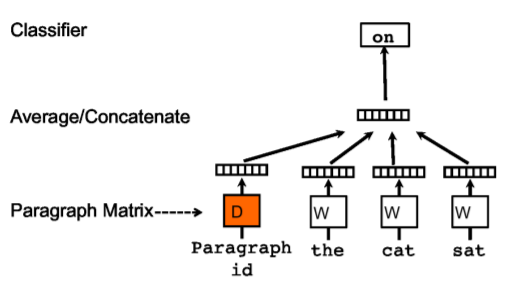
\includegraphics[width=0.70\textwidth]{images/doc2vec-arch.PNG}
    \caption{The DM-PV model.}
    \label{fig:doc2vec-arch}
\end{figure}
The distributed memory model of paragraph vectors, also refered to as DM-PV, attemps to generalize the abilities of CBOW to variable-length documents.
In DM-PV, every document is mapped to a unique vector represented by a row in a matrix $\textbf{D} \in \mathbb{R}^{M \times N}$, where 
$M$ denotes the number of documents. 
As before, every word is also mapped to a vector in an input matrix $\textbf{W} \in \mathbb{R}^{V \times N}$ and an output matrix $\textbf{W'} \in \mathbb{R}^{N \times V}$, respectively. 
The only difference between DM-PV and CBOW is that the document vector $d_{j}$ that 
contains the words is asked to contribute to the prediction task 
by being integrated into the hidden state in Equation (\ref{eq:hidden_state}).
See Figure \ref{fig:doc2vec-arch} for a visual representation. 
Thus, the new hidden state is computed as follows: 
\begin{equation}
    \textbf{h} = d_j + \frac{1}{C}(v_1 + v_2 + \hdots + v_c ), \:
    \textbf{h} \in \mathbb{R}^{N}.
\end{equation}
The document vector can be thought of as another word. It acts as a memory that remembers 
what is missing from the current context, i.e the document's topic. 
Note that the document vector is shared across all contexts $v_1 + v_2 + \hdots + v_c$ 
generated from the same document, but not across documents.
Conversely, the word vector matrices $\textbf{W}$ and $\textbf{W'}$ are shared across documents. 
During backpropagation, the derivative of the cost function with respect to the target document vector 
\begin{equation}
\frac{\partial H}{\partial d_{j}}
\end{equation}
is computed as well, thus pushing documents with similar words towards those words and therefore, towards each other.  
\subsection{Inference}
So far, we've only considered the case of training the algorithm in order to create numeric representations for \textbf{previously seen} documents.
But how do we generate such representations for unseen documents? This problem is addressed in the \textbf{inference stage}.\\
Given is an unseen document $d$. A randomly-initialized vector is added to our model's weight matrix $\textbf{D}$.
That vector represents the document vector for $d$. 
The vector for $d$ is updated by gradient descending on $\textbf{D}$ for $i$ epochs while keeping $\textbf{W}$, $\textbf{W'}$ and their gradients fixed.
The number of epochs to descent on $d$ should match the number of epochs used during training. 

%\printbibliography[heading=bibintoc, filter={bookorarticleormisc}, title={Scientific references}]
%\printbibliography[heading=bibintoc, keyword={online}, title={Online references}]\clearpage
%\printbibliography[heading=bibintoc, keyword={image}, title={Image references}]\clearpage
\end{document}
